\subsection{Posterior Inference under the Extended Model}
\label{res:post_contour}
Figure~\ref{fig:contour} displays the joint posterior distribution of $(\lambda, A)$, together with the MAP estimate and the corresponding HPD regions. The posterior mode is located at $\lambda \approx 0.0138$ and $A = y_{\max} \approx 179.45$ months, indicating that the estimate of $A$ coincides exactly with the longest observed tenure in the data. This suggests that the posterior inference of $A$ is strongly driven by the boundary constraint rather than by additional evidence from the data.

First, the posterior distribution of $\lambda$ is highly concentrated, with a relatively narrow range. This shows that the event rate parameter $\lambda$ is primarily determined by the observed event times and can therefore be estimated with high precision. By contrast, the uncertainty associated with $A$ is substantially larger.

Second, the HPD regions exhibit a clear truncation effect at the boundary $A = y_{\max}$. Since the model enforces $A \geq y_{\max}$, the posterior mass is forced against this boundary, creating a sharp cutoff on the left. As a result, the MAP point falls exactly on the boundary, while the 86.5\% HPD region extends almost entirely upward along this edge, forming a one-sided expansion rather than a symmetric spread around the mode, as would be typical under a Gaussian distribution. In other words, the uncertainty in $A$ is essentially about “how much larger than $y_{\max}$ it could be,” rather than about symmetric fluctuations around the MAP.

A closer comparison of the HPD regions further reinforces this interpretation: if the posterior were approximately Gaussian and independent, the 39.3\% and 86.5\% regions would resemble concentric ellipses. In contrast, here the outer region expands asymmetrically in the $A$ direction and clings to the boundary, revealing a boundary-driven skewness rather than Gaussian-like symmetric tails. The slight tilt of the contour also suggests a weak dependence between $\lambda$ and $A$, reflecting the fact that the censoring window and event rate jointly shape the observed data. However, this dependence is secondary compared with the strong boundary effect dominating the inference for $A$.

This observation naturally motivates the marginalization analysis in the next section. By integrating out $A$, we can check whether the extended formulation remains consistent with the baseline exponential model in terms of $\lambda$, thereby clarifying to what extent the introduction of $A$ truly alters—or preserves—the original inferential structure.
\begin{figure}[H]
    \centering
    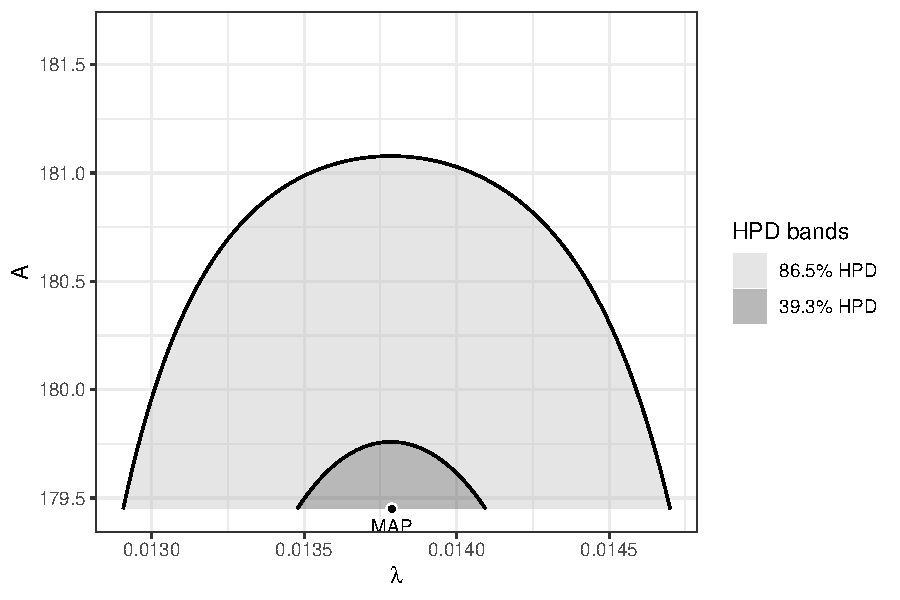
\includegraphics[height=9cm, width=0.65\textwidth]{images/post_contour.pdf}
    \caption{{\small Joint posterior $p(\lambda,A\mid\mathcal D)$ with 39.3\%/86.5\% HPD contours and MAP (black).}}
    \label{fig:contour}
\end{figure}


\subsection{Marginalization and Consistency Check}
\label{res:marginal}
Building on the boundary-driven geometry in Section~\ref{res:post_contour}, we now ask whether introducing $A$ changes inference on $\lambda$ once we focus on $\lambda$ alone. Figure~\ref{fig:marginal} compares the marginal posterior of $\lambda$ obtained from the extended model (blue; integrating out $A$ on the grid) with the analytic posterior from the baseline exponential model that does not include $A$ (red).

The two curves are visually indistinguishable across the entire support: the peak location, peak height, and tail decay coincide to plotting precision, and the associated credible intervals match to numerical accuracy. This confirms a key point for practice: Inference on $\lambda$ is preserved after introducing $A$. In the extended model, $A$ behaves as a (predictive) nuisance parameter: it is crucial for generating realistic fake data and for describing the observation window, but it does not alter the posterior for the event-time rate $\lambda$.

This empirical agreement is exactly what the factorization of the likelihood predicts (see Section~\ref{边际化章节}): the $\lambda$-dependent and $A$-dependent terms separate, so integrating over $A$ contributes only a normalizing constant that does not depend on $\lambda$. Consequently, the boundary-driven skewness seen along the $A$ direction in Section~\ref{res:post_contour} does not propagate into the marginal for $\lambda$.

\begin{figure}[H]
    \centering
    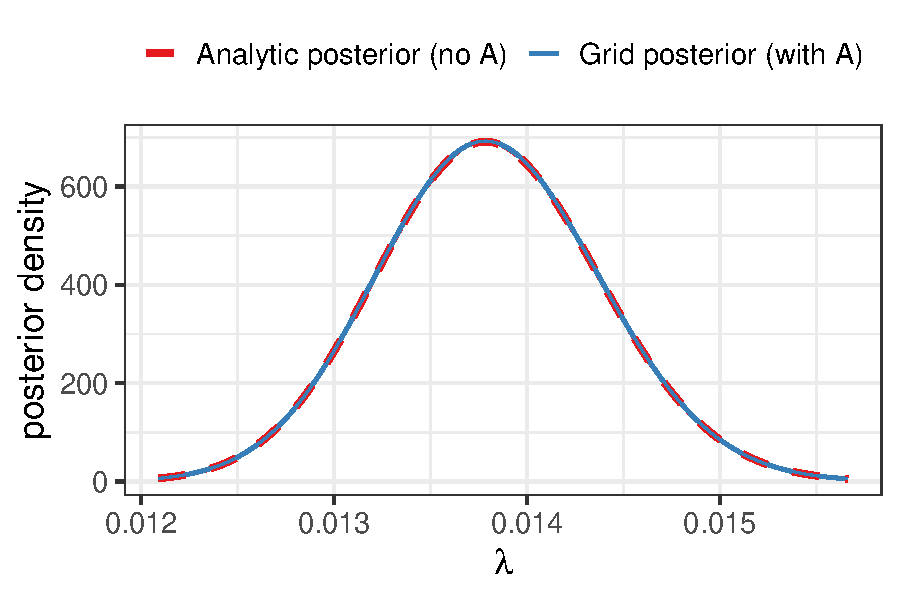
\includegraphics[height=6cm, width=0.7\textwidth]{images/lambda_marginal_compare.pdf}
    \caption{{\small Marginal posterior of $\lambda$ under the extended model (blue, obtained by integrating out $A$) versus the analytic posterior under the baseline exponential model (red).}}
    \label{fig:marginal}
\end{figure}
To further examine the stability of the marginal posterior for $\lambda$, we compared two sharply different priors for $A$: a weakly informative uniform prior $[y_{\max}, y_{\max}+500]$ and a truncated normal prior centered around $y_{\max}+50$. As shown in Figure~\ref{fig:diff_A_marginal}, despite the substantial difference in prior shapes, the resulting marginal posteriors for $\lambda$ are virtually identical.

This robustness is fully consistent with the theoretical result in equation~\eqref{eq:47} in Section~\ref{边际化章节}. As long as the prior for $A$ is independent of $\lambda$, integrating out $A$ contributes only a constant factor. Consequently, the marginal posterior of $\lambda$ is determined entirely by its likelihood and remains unaffected by the specific form of the prior on $A$.
\begin{figure}[H]
    \centering
    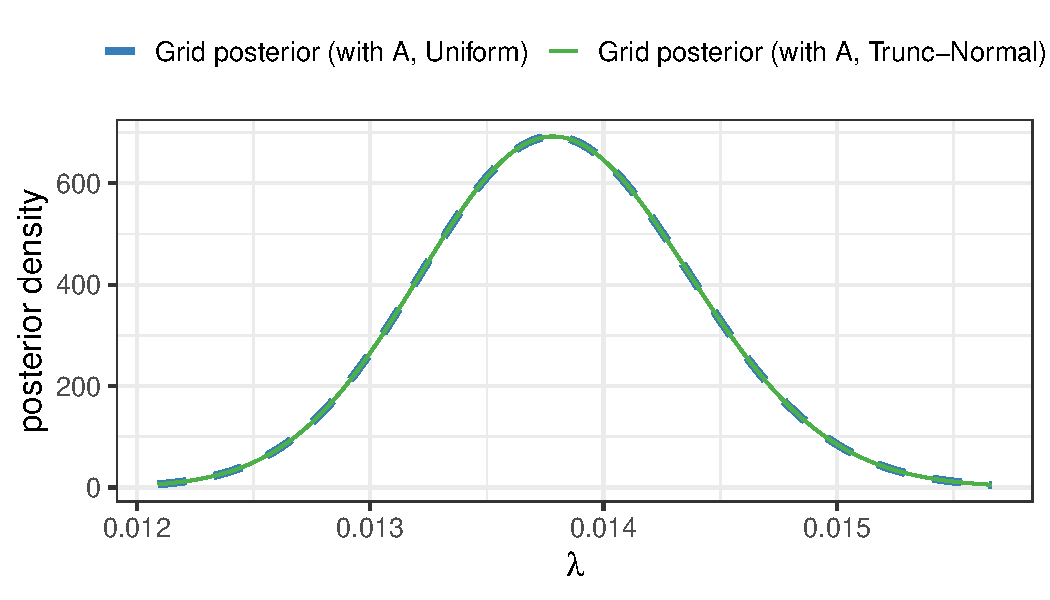
\includegraphics[height=6cm, width=0.75\textwidth]{images/diff_A_prior_marginal_compare.pdf}
    \caption{{\small Marginal posterior of $\lambda$ under two priors for $A$: uniform $[y_{\max}, y_{\max}+500]$ (blue) and truncated normal near $y_{\max}+50$ (green).}}
    \label{fig:diff_A_marginal}
\end{figure}

\subsection{Baseline Model Fit and Limitations}
\label{res:baseline_ecdf}
While Section~\ref{res:marginal} showed that marginalizing out $A$ preserves the baseline inference on $\lambda$, such consistency does not guarantee that the baseline model itself adequately reflects the data. To further assess its validity, we first perform a simulation-based model check. Specifically, we generated pseudo-data with a fixed value $\lambda=0.05$ and refitted the exponential model. As shown in Table~\ref{tab:post-ci}, the posterior mean (0.053) and 95\% CrI [0.0496, 0.0567] successfully recover the true value, indicating that the model is structurally sound. For completeness, the full posterior histogram is provided in Supplementary Figure~\ref{fig:posterior_s1}.
\begin{table}[H]
\centering
\caption{{\small Posterior summaries and 95\% credible intervals (simulation-based model check)}}
\label{tab:post-ci}
\small
\begin{tabular}{lccccc}
\toprule
{Parameter} & {Mean} & {2.5\%} & {97.5\%} & {$n_{\text{eff}}$} & {Rhat} \\
\midrule
$\lambda$   & 0.0531 & 0.0496 & 0.0567 & 1113 & 1.000 \\
\bottomrule
\end{tabular}
\end{table}
Having established that the baseline model is structurally coherent, we next examine its adequacy when applied to real data. In the posterior predictive model checking of the baseline specification, the true value of the observation-window parameter $A$ is unknown. Section~\ref{Impact of A} illustrated the distributional consequences of three candidate values, $A=30, \,200,$ and $1000$ months. Here, we concentrate on the two extremes, $A=30$ and $A=1000$, to examine how the baseline model behaves under contrasting window lengths. Posterior predictive checks under these settings yield the empirical cumulative distribution functions (ECDFs) shown in Figures~\ref{fig:ppc_a30}~\ref{fig:ppc_a1000}, which are compared against the real data.

\textbf{Case $A=30$ (Figure~\ref{fig:ppc_a30}):} For both event times and censored durations, the predictive ECDFs rise sharply in the early period and deviate strongly from the observed curves. The simulated curves are nearly linear, approximating a uniform distribution, which implies that the model expects most individuals to either fail or be censored within a short window. This eliminates the exponential decay pattern visible in the real data. The corresponding counts are events = 184 and censored = 945 (Table~\ref{tab:modelcheck_counts}), which differ drastically from the real data (events = 571, censored = 558), with the censored proportion being far too high. The histograms (Figure~\ref{fig:fake-hist_a30} in Section~\ref{Impact of A}) likewise show that durations are artificially compressed into the 0–30 month range. This indicates that when $A$ is too small, the model mechanically forces most individuals into “premature censoring,” leading to a breakdown of the fit.

\textbf{Case $A=1000$ (Figure~\ref{fig:ppc_a1000}):} The predictive ECDFs appear superficially closer to the real curves, particularly in the tail, where the discrepancy is less obvious. However, the corresponding counts (events = 1055, censored = 74) are highly imbalanced, with almost all individuals predicted to experience the event. The histograms (Figure~\ref{fig:fake-hist_a1000}) confirm that durations are stretched into implausibly long tails. This explains why the ECDFs look deceptively close to the observed data: with almost no censored individuals, nearly all samples are forced onto the “event curve,” which smooths the overall shape. Yet this apparent fit is spurious, as it distorts the censoring mechanism and fails to capture the structural properties of the data.

\begin{table}[H]
\centering
\caption{{\small Event and censoring counts in real and simulated datasets (model checking)}}
\label{tab:modelcheck_counts}
\small  
\begin{tabular}{lcc}
\toprule
\textbf{Dataset} & \textbf{Censoring ($0$)} & \textbf{Events ($1$)} \\
\midrule
Real data        & 558  & 571  \\
Simulated ($A=30$)   & 945  & 184  \\
Simulated ($A=1000$) & 74   & 1055 \\
\bottomrule
\end{tabular}
\end{table}

\begin{figure}[H]
    \centering
    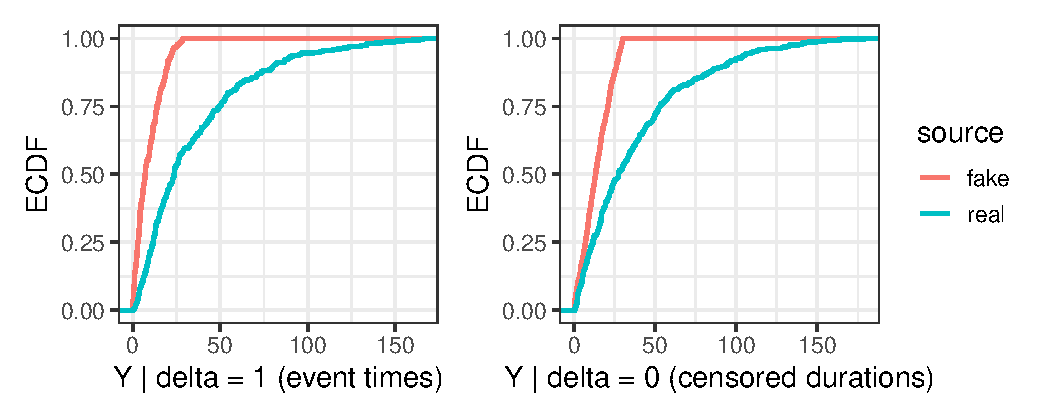
\includegraphics[height=4cm, width=0.8\textwidth]{images/ppc_two_a30.pdf}
    \caption{{\small Posterior predictive ECDFs of event times (left) and censored durations (right) under fixed $A=30$.}}
    \label{fig:ppc_a30}
\end{figure}

\begin{figure}[H]
    \centering
    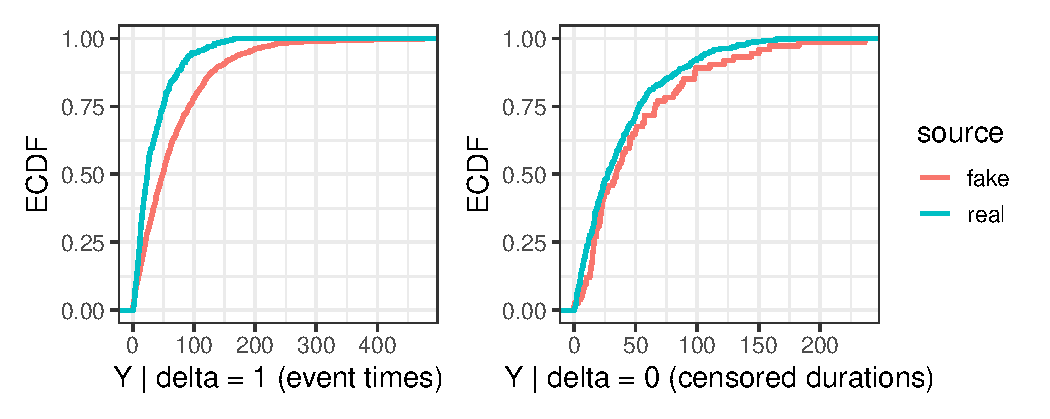
\includegraphics[height=4cm, width=0.8\textwidth]{images/ppc_two_a1000.pdf}
    \caption{{\small Posterior predictive ECDFs of event times (left) and censored durations (right) under fixed $A=1000$.}}
    \label{fig:ppc_a1000}
\end{figure}
These results highlight a structural mismatch: the baseline exponential model cannot reproduce the censoring pattern observed in the data. To address this, we turn to the extended model with the observation-window parameter $A$ and evaluate its performance through posterior predictive model checking.


\subsection{Posterior Predictive Model Checking (Extended Model)}

The baseline model failed to reproduce the censoring structure, underscoring the need for an extended specification. By introducing the observation-window parameter $A$, the model is able to capture this structural feature. The joint posterior yields MAP estimates of $\lambda \approx 0.0138$ and $A \approx 179$, which are consistent with the intuitive setting of $A \approx 200$ discussed in Section~\ref{Impact of A}. This consistency illustrates how the Bayesian framework can formalize and refine prior intuition.

Posterior predictive checks based on the MAP estimates demonstrate clear improvements in reproducing the observed data. For event times, the MAP-simulated ECDF (Figures~\ref{fig:ppc_map}) aligns closely with the empirical curve, especially in the early growth phase, indicating that the model captures the dynamics of event occurrence accurately. In contrast, the $A=1000$ specification produces a noticeably flatter curve, reflecting an underestimation of early event rates, even though its tail appears superficially smooth.

For censored durations, the MAP fit is again more reasonable. While some discrepancies remain, the distributional structure is much closer to the real data: censored observations are spread across the 0–180 month range with a smooth decline in frequency, as shown in the histogram~\ref{fig:fake_map}. This avoids the over-compression seen under $A=30$ as well as the near-elimination of censoring under $A=1000$, where apparent curve alignment arises only from proportional effects rather than a faithful representation of the censoring mechanism.

Overall, the MAP-based extended model not only reproduces the shape of the ECDFs but also recovers the structural balance between events and censoring. These results highlight the substantive improvement of the extended specification over the baseline model.
\begin{figure}[H]
    \centering
    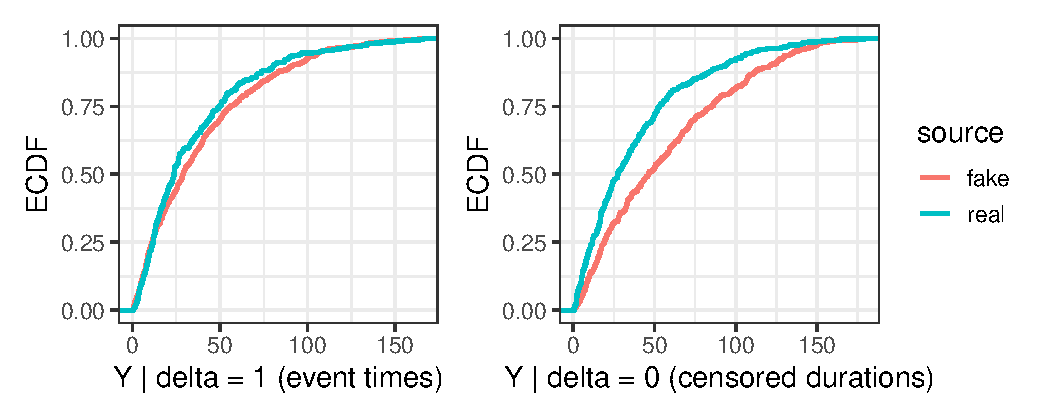
\includegraphics[height=4cm, width=0.8\textwidth]{images/ppc_two_map.pdf}
    \caption{{\small Posterior predictive ECDFs of event times (left) and censored durations (right) under the MAP estimates ($\lambda \approx 0.0138, A \approx 179$)}}
    \label{fig:ppc_map}
\end{figure}

\begin{figure}[H]
    \centering
    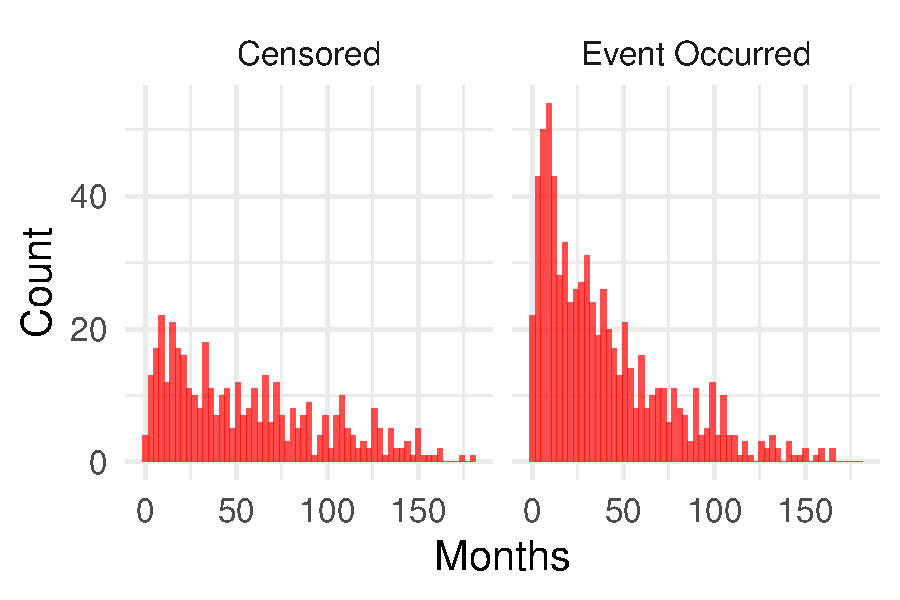
\includegraphics[height=5cm, width=0.6\textwidth]{images/fake_duration_hist_Apost.pdf}
    \caption{{\small Posterior predictive histograms of event times (right) and censored durations (left) under the MAP estimates ($\lambda \approx 0.0138, A \approx 179$)}}
    \label{fig:fake_map}
\end{figure}